%------------------------------------------------------------------------------
% Beginning of outline.tex
%------------------------------------------------------------------------------
\documentclass{article}
\usepackage{graphicx}
\usepackage{enumitem}
\usepackage{url}
\usepackage{amsthm}
\usepackage{hyperref}
\usepackage{mathtools}
\usepackage{amssymb}
\usepackage{float}
\usepackage{amsmath}
\usepackage{setspace}

%\singlespacing
\doublespacing

\theoremstyle{definition}
\newtheorem{defn}{Definition}[subsection] % definition numbers are dependent on theorem numbers
\newtheorem{thm}{Theorem}[subsection]

%    Absolute value notation
\newcommand{\abs}[1]{\lvert#1\rvert}
\newcommand{\qi}{\text{\textbf{i}}}
\newcommand{\qj}{\text{\textbf{j}}}
\newcommand{\qk}{\text{\textbf{k}}}
\newcommand{\qq}{\text{\textbf{q}}}
\newcommand{\qr}{\text{\textbf{r}}}
\newcommand{\qu}{\text{\textbf{u}}}


\begin{document}
\pagenumbering{gobble}
%\nocite{*}
\title{Rotations in 3 Dimensions with Quaternions}
\date{\today}
%    Information for first author
\author{Sean Turner}
\maketitle

\begin{figure}[H]
\centering
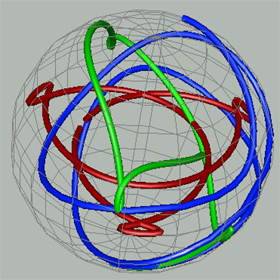
\includegraphics[width = .65\textwidth]{Figures/quaternion_map}
\end{figure}

\newpage
\pagenumbering{roman}
\tableofcontents
\listoffigures
\newpage
\pagenumbering{arabic}
\begin{abstract}
\noindent William Rowan Hamilton first described quaternions in 1843.
Quaternions are used to describe transformation in 3-d space and have many applications in aeronautics, robotics, and computer graphics.
This manuscript will provide a brief overview of quaternions and spatial geometries, specifically relating to algebra, geometry, and differential calculus.
This will be followed by a comparision between quaternions, euler angles, and rotational matrices, and then a discussion of their applications.
\end{abstract}

\section{Introduction}
Nobody knows how long vectors have been used in mathematics.
Some speculate that the parallelogram method for addition of vectors was lost in a work of Aristotle.
However quaternions, often defined as the quotient of two vectors, were not described until 1843 by William Rowan Hamilton.
Quaternions are now extensively used in aeronautics and computer graphics for their advantages over tradional transformtion methods.


\subsection{History of Quaternions}

On October 17, 1843, William Rowan Hamilton wrote a letter to his friend John t. Graves, Esq. on the subject of ``a very curious train of mathematical speculation."
The letter details his ``theory of quaternions", and follows his mathematical reasoning behind the development of his ``quaternions."
The day before, while walking across the Royal Canal in Dublin, Hamilton had the idea for the formula of quaternions as shown below in Equation \ref{eq:quat}.
\begin{equation}
\label{eq:quat}
i^2 = j^2 = k^2 = ijk = -1
\end{equation}
This equations and its implications will be investigated in Section \ref{sec:disc}.
The letter was only a few pages long, but it quite thorough in its' scope, and was eventually published in the \textit{London, Edinburgh, and Dublin Philosophical Magazine and Journal of Science} the following year in 1844.
Shortly after Hamilton's death in 1865, his son edited and published the longest of Hamilton's books, at over 800 pages.
Titled \textit{Elements of Quaternions}, this book was the go-to book on quaternions for several decades.
The wake of Hamilton's exploration into quaternions led to research associations like the Quaternion Society who described themselves as an ``International Association for Promoting the Study of Quaternions."

\subsection{Basic Geometric Transformations}
\label{sub:geo}

The primary topic of this manuscript is the application of quaternions to rotations in 3D space, so some terms will be defined here.
There are two methods of transformation: translation and rotation \cite{animation}.

\begin{defn}[Translation]
A \textit{translation} is a point in space moved from one position to another.
Let a point $P \in \mathbb{R}^3$ be denoted as $(x,y,z), x,y,x \in \mathbb{R}$ and the translation by a vector $(\Delta x, \Delta y, \Delta z)$.
Then the new position $P^\prime$ is $(x + \Delta x, y + \Delta y, z + \Delta z)$.
There is only one translation vector that takes $P$ to $P^\prime$.
\end{defn}

\noindent A \textit{rotation} can be defined in multiple ways.
The following definition is given by Euler, and will be used here.

\begin{defn}[Euler's Definition of Rotation]
Let $O, O^\prime \in \mathbb{R}^3$ be two orientations.
Then there exists an axis $l \in \mathbb{R}^3$ and an angle of rotation $\Theta \in [-\pi, \pi]$ such that $O$ yields $O^\prime$ when rotated $\Theta$ about $l$.
\end{defn}

\noindent It is important to distinguish between \textit{orientation} and \textit{rotation}.
Orientation here is the normal vector to an object in 3D space.
A rotation comprised of an axis and angle of rotation.
Unlike the translation between two points, the rotation between two orientations in 3D space is not unique.
\\ \\
\noindent Section \ref{sec:disc} will define and discuss quaternions in detail.
Section \ref{sec:comp} will compare quaternions and alternate methods of expressing rotations, while Section \ref{sec:app} will discuss real world applications.
Section \ref{sec:conc} will conclude the report.


\section{Discussion}
\label{sec:disc}
The quaternion equation was briefly introduced in Equation \ref{eq:quat}.
The following definition is a rigorous definion that follows from that equation.
\begin{defn}[Quaternion]
A \textit{quaternion} is a number of the form $$a + b\qi + c\qj + c\qk $$ where a, b, c, and d are real numbers, \qi, \qj, \qk, are square roots of -1, and \qi\qj\qk = -1.
\end{defn}
\noindent The following section will describe quaternions in more depth, specifically related to algebra, geometry, and differential calculus.
\subsection{Algebra \& Quaternions}
The addition and subtraction of quaternions is the same as 4D vector addition.
That is, adding quaternions is simply separately adding the coefficients of \qi, \qj, \qk.
For example, $$ (1 + 2\qi + 3\qj + 4\qk) + (-2 + 3\qi - 1\qj + 4\qk) = -1 + 5\qi + 2\qj + 8\qk$$
\noindent Multiplication is a little more involved.
Clearly, since \qi, \qj, and \qk  are square roots of -1, it is true that $\qi^2 = \qj^2 = \qk^2 = -1$.
However, it is not so clear what, for example, $\qi\qj$ is.
We know that $\qi\qj \neq -1$ because $\qi \qj \qk = -1$, and $\qk \neq 1$.
To find $\qi\qj$ we must use Equation \ref{eq:quat} as shown: $$ \qi\qj = -\qi\qj(-1) = -\qi\qj\qk^2 = -(\qi\qj\qk)\qk = -(-1)\qk = \qk$$
It is important to note that quaternion multiplication is not commutative, since $ \qi\qj = \qk \neq \qj\qi = -\qk $.
A full table of the quaternion relationships between \qi, \qj, and \qk$ $ are shown below in Table \ref{tab:quat}:
\begin{table}[H]
\centering
\caption{Quaternion Characteristics}
\label{tab:quat}
\begin{tabular}{|l|l|l|l|}
\hline
 & \qi & \qj & \qk \\ \hline
\qi & \text{\textbf{-1}} & \qk & -\qj \\ \hline
\qj & -\qk & \text{\textbf{-1}} & \qi \\ \hline
\qk & -\qj & \qi & \text{\textbf{-1}} \\ \hline
\end{tabular}
\end{table}

Quaternion multiplication is not commutative as shown above, but other algebraic properties are satisfied as shown in Theorem \ref{thm:mult}

\begin{thm}
\label{thm:mult}
\begin{enumerate} \textit{Properties of Quaternion Multiplication}
	\item Associativity: $\qq ( \textbf{r} \textbf{s}) = (\textbf{q} \textbf{r}) \textbf{s}$
	\item Distributivity: $\qq (\textbf{r} + \textbf{s}) = \textbf{q} \textbf{r} + \textbf{q} \textbf{s}$
	\item Inverses: $\forall$ quaternions $\qq \neq 0$, $\exists$ a quaternion $\textbf{r}$ s.t. $\textbf{qr} = 1$
	\item Cancellation: If $\textbf{qr}=\textbf{qs}$, then $\textbf{r} = \textbf{s}$
\end{enumerate}

\end{thm}

\noindent When quaternions are written in the form $\qq = a + b\qi + c\qj + d\qk$, they are said to be in \textit{Cartesian form}, similar to the method of displaying a complex number in the form $a + bi$.
Just as we can separate a complex number into real and imaginary parts, so we can split a quaternion \textbf{q} into a \textit{scalar} part $S\qq = a$ and a \textit{vector} part $V\qq = b\qi + c\qj + d\qk$.
We can also define the \textit{conjugate} of a quaternion as $$ \qq^* = S\qq - V\qq = a - b\qi - c\qj - d\qk,$$ and the \textit{absolute value} of \qq$ $ as $$ \abs{\qq} = \sqrt{a^2 + b^2 + c^2 + d^2}.$$


\subsection{Geometry \& Quaternions}

\subsection{Differential Calculus \& Quaternions}


\section{Comparison}
\label{sec:comp}
\subsection{Other Non-Euclidean Transformation Methods}
	\begin{enumerate}[label={(\alph*)}]
		\item Key Definition 5: Euler Angles
		\item Key Definition 6: Rotation Matrix
	\end{enumerate}

\subsection{Comparisions Between Methods}
	\begin{enumerate}[label={(\alph*)}]
		\item Euler Angles and Quaternions
		\item Rotation Matrices and Quaternions
	\end{enumerate}


\section{Applications}
\label{sec:app}
\subsection{Aeronautics \& Quaternions}
Aeronautics often deal with the problem of rotation.
An airplane has an ``internial frame", which needs to be corresponded to the `` body frame."
A common way to represent rotation on an airplane is with the following convention:
\begin{figure}[H]
\centering
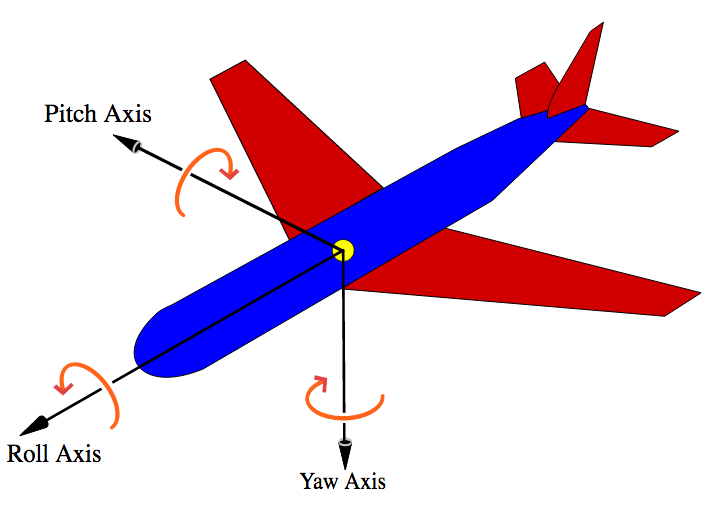
\includegraphics[width = .75\textwidth]{Figures/plane.png}
\caption{Roll, Pitch, and Yaw}
\label{fig:cycle}
\end{figure}
Roll, pitch, and yaw are simply Euler angles.
When flying a small plane, and rotating about a single axis, it may be easier to use Euler angles.
However, many large commerical airlines use computer assisted flight with many maneuvers done on autopilot.
Complicated rotations may be represented as an arbitrary rotation about an arbitrary axis, the perfect use case for quaternions.
There is another reason to use quaternions rather than rotation matrices when flying.
Rotations in 3D space can be thought of as a three gimbal system, where a gimbal is `` a pivoted support that allows the rotation of an object about a single axis.''
Figure \ref{fig:gimbal} shows an example of a 3-axis gimbal system.
\begin{figure}[H]
\centering
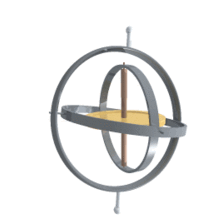
\includegraphics[width = .75\textwidth]{Figures/gimbal.png}
\caption{A 3-Axis Gimbal System}
\label{fig:gimbal}
\end{figure}
 This is essentially a visualization of Euler angles, where the deviation from the traditional 3-axis orientation can be used to keep track of the orientation of the system.
 Gimbals are commonly used in gyroscopes, aeronautics, and rocket systems.
 Gimbals in a 3-axis configuration have 3 degrees of freedom.
 A phenomenon can occur where gimbals end up in the same plane, and you lose a degree of freedom.
 Figure \ref{fig:gimlock} shows a locked gimbal system.

 \begin{figure}[H]
 \centering
 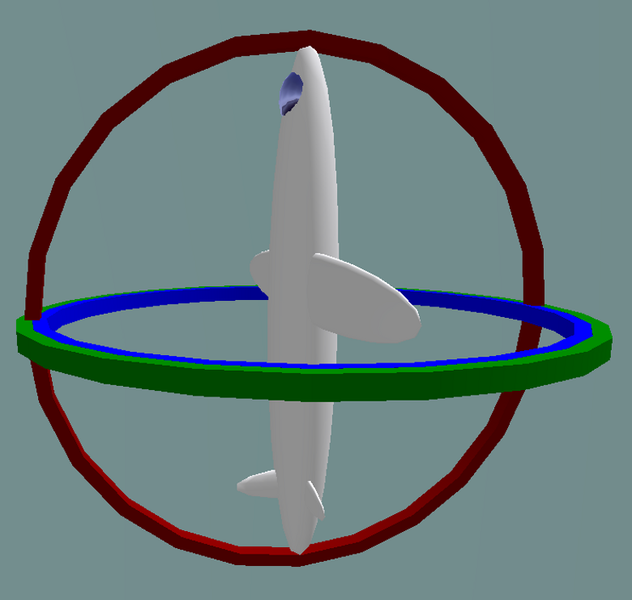
\includegraphics[width = .75\textwidth]{Figures/gimbal_lock.png}
 \caption{Roll and Yaw Gimbal Locked System}
 \label{fig:gimlock}
 \end{figure}

 In the above figure, the roll and yaw axes are now represented with a single gimbal.
 If the plane is told to rotate roll or yaw, the rotation is applied to the same axis.
 The only way to get out of gimbal lock is to rotate about the single gimbal.
 Gimbal lock is a property of Euler angles and rotation matrices.
 Here is the rotation matrix for the ($\alpha, \beta, \gamma$) angles that we did not calculate earlier.

 $$
 R =
 \begin{bmatrix}
 \text{cos }\beta \text{ cos }\gamma 																& -\text{sin }\gamma \text{ cos }\beta & \text{sin }\beta \\
 \text{sin }\beta \text{ cos }\alpha  \text{ cos }\gamma + \text{cos }\alpha \text{ sin }\gamma 	& - \text{sin }\gamma \text{ sin }\alpha \text{ sin }\beta + \text{cos }\alpha \text{ cos }\gamma & -\text{cos }\beta \text{ sin }\alpha \\
 -\text{sin }\beta \text{ cos }\gamma \text{ cos }\alpha + \text{sin }\alpha \text{ sin }\gamma 		& \text{sin }\gamma \text{ sin }\beta \text{ cos } \alpha + \text{ sin }\alpha \text{ cos } \gamma & \text{cos } \alpha \text{ cos } \beta
 \end{bmatrix}
 $$

Let us take $\beta= \frac{\pi}{2}$.
This results in the following rotation matrix:

$$
R =
\begin{bmatrix}
0 & 0 & 1 \\
\text{cos }\alpha  \text{ cos }\gamma + \text{cos }\alpha \text{ sin }\gamma 	& - \text{sin }\gamma \text{ sin }\alpha + \text{cos }\alpha \text{ cos }\gamma& 0 \\
 -\text{cos }\gamma \text{ cos }\alpha + \text{sin }\alpha \text{ sin }\gamma 		& \text{sin }\gamma \text{ cos } \alpha + \text{ sin }\alpha \text{ cos } \gamma  & 0
\end{bmatrix}
$$

Using trigonometric identities, we can simplify this rotation matrix as shown below.

$$
R =
\begin{bmatrix}
0 & 0 & 1 \\
\text{sin }(\alpha + \gamma) 	& \text{cos }(\alpha + \gamma) & 0 \\
-\text{cos }(\alpha + \gamma) 	& \text{sin }(\alpha + \gamma)   & 0
\end{bmatrix}
$$

Clearly, changing $\alpha$ or $\gamma$ has the same affect.
The gimbal is in effect, ``locked."
To fix this and get out of the gimbal lock, $\beta$ must be rotated first.
This is a problem inherant to Euler angles and their use in rotation matrices, but does not affect quaternions.

\subsection{Computer Graphics \& Quaternions}

Computer graphics, and specifically computer animation, rely on quaternions to express rotation between orientations.
Several game engines come with the ability to use quaternions on the back end.
The 2D and 3D cross-platform game engine called ``Unity", has instructions for coders and animators for implementing quaternions in their projects.
There are several reasons that quaternions offer advantages that have already been discussed, namely computation time, memory needed to represent a single rotation, and avoiding gimbal lock.
There is one other reason that quaternions offer and advantage to rotation matrices.
To investigate this, let us look at the basics of animation.
\subsubsection{Animation}
Animation relies on simulating three dimensional objects on a rigid frame and projecting them onto a 2D surface.
Tranformations (rotations and translations) are used to move objects between orientations and positions.
Methods such as spherical interpolation can be used to control the position of infinitely distant light sources, or to model features on a globe.
Let's say we are trying to animate a health bar in a video game.
We might pick several points that we want the bar to go through, and then perform a linear interpolation to fill in the points between.
It would not be too hard to pick some points that are evenly spaced apart, so that the movement does not appear to be jerky when rendered in an animation.
This method, shortened to \textit{lerp}, is commonly used for interpolating linear distance or velocity.
However, \textit{lerp} does not work well when trying to do spherical interpolation, shortened to \textit{slerp}. \cite{animation}
\\ \\ Imagine we are trying to animate an object about arbitrary axis, $\beta$, and by an arbitrary angle, $\theta$.
We have discussed several methods for obtaining the rotation about $\beta$ by $\theta$.
We could, for example, compute several different Euler angles and then individually rotate about each axis to achieve the desired rotation.
However, despite being valid mathematically, this would look pretty odd when animated.
Another solution might be to rotate using the quaternion, or rotation matrix, but linearly interpolated.
This is a natural rotation, but might appear jerky because the interpolation is not smooth, and if using a rotation matrix, we could still run into the problem of gimbal lock.
The solution is to use \textit{slerp} to animate a smooth interpolation with quaternions.
This achieves the desired smoothness, without fear of gimbal lock.
The mechanics behind \textit{slerp} are outside of the scope of this paper, but it works by keeping a constant speed.
The geometric formula for \textit{slerp}, as detailed by Ken Shoemaker, is given below in Equation \ref{eq:slerp}.

\begin{equation}
	Slerp(p_0, p_1, t) = \frac{sin[(1-t)\Omega]}{sin\Omega}p_0 + \frac{sin[t\Omega]}{sin\Omega}p_1
	\label{eq:slerp}
\end{equation}

When using Slerp to interpolate quaternions, it produces a uniform angular velocity around a rotation axis.
The same equation using quaternions is shown below in Equation \ref{eq:slerp2}.

\begin{equation}
	Slerp(q_0, q_1, t) = (q_1q_0^{-1})^tq_0
\label{eq:slerp2}
\end{equation}

To investigate the application of slerp, some MATLAB code was written to interpolate a vector rotation.
This code for this is shown below.

\begin{verbatim}
	v = [1 .5 1]; % vector
	iterations = 100;
	p = [1 0 0 0]; % initial quaternion, does not rotate
	q = [1 0 1 0]; % Random Quaternion
	quat2eul(q) %Makes visualization easier, return euler angles in ZYX

	pn = quatnormalize(p); % normalization to unit quaternions
	qn = quatnormalize(q);
	qi = quatinterp(pn,qn,1/iterations,'slerp'); % performs interpolation between extremes

	plot3([0 v(1)], [0 v(2)], [0 v(3)]); % plot initial vector
	grid on;
	hold on;
	r = quatrotate(p,v); % doesn't rotate, but initializes r

	for i = 1:iterations % loops over iterations and applies rotation about quaternion
	    r = quatrotate(qi, r);
	    plot3([0 r(1)], [0 r(2)], [0 r(3)]);
	end

	rotate3d; % allows for click and drag in 3d plot
\end{verbatim}

Using an iteration value of 2 gives the following result.

\begin{figure}[H]
\centering
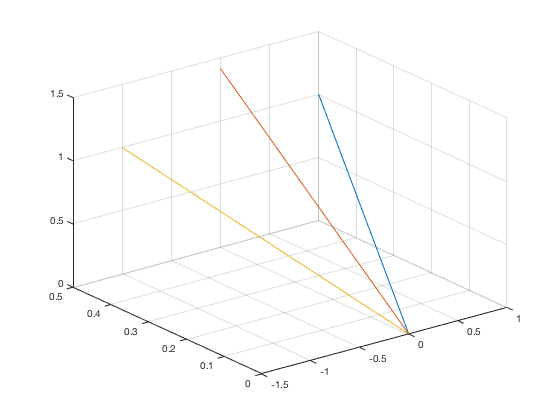
\includegraphics[width = .75\textwidth]{Figures/slerp2.png}
\caption{Slerp Example with 3 Iterations}
\label{fig:slerp3}
\end{figure}

The quaternion used in the code rotates the vector about the y-axis by an angle of $90^\circ$.
Notice the spherical interpolation of the second vector.
Using an iteration value of 100 yields the following plot.


\begin{figure}[H]
\centering
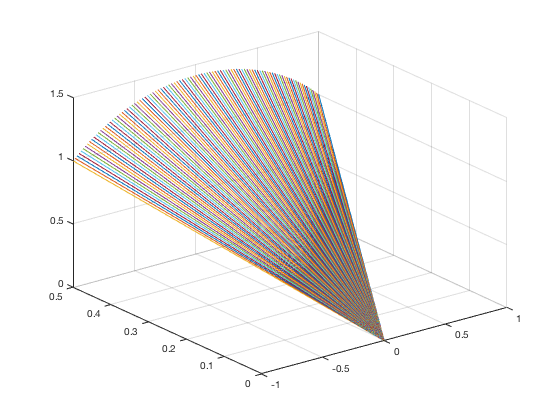
\includegraphics[width = .75\textwidth]{Figures/slerp100.png}
\caption{Slerp Example with 100 Iterations}
\label{fig:slerp100}
\end{figure}

Here the spherical interpolation is more clearly noticable.
The MATLAB code is easy to use, and performs the necessary interpolation quickly.


\section{Conclusion}
\label{sec:conc}
This paper details several different transformation methods for rotation in three dimensions.
Euler angles, rotation matrices, and quaternions were all described, and compared, and the conversions between them were presented.
Overall, quaternions offer better usability for almost every application, except in applications were translations are also needed.
Quaternions have uses in aeronautics, robotics, and computer graphics.
They prevent gimbal lock, a phenomenon whereby three degrees of freedom becomes two degrees of freedom.
Quaternions are also used for spherical interpolation, also known as \textit{slerp}.
MATLAB code was used to investigate quaternions and slerp.


\newpage
\bibliography{references}
\bibliographystyle{amsplain}

\end{document}

%------------------------------------------------------------------------------
% End of outline.tex
%------------------------------------------------------------------------------
